\documentclass[gray]{beamer}
%\setbeamertemplate{headline}{\scriptsize{\vspace*{0.3cm}\hspace*{0.3cm}\insertframenumber}} 

\setbeamertemplate{footline}[page number]{}

\setbeamertemplate{navigation symbols}{}

\begin{document}
\title{Large Scale and High Performance NoSQL Databases in Web Applications}  
 
\author{Mateusz Bilski, mateusz.bilski@gmail.com \\ Ireneusz Kawalec, ireneusz.kawalec@gmail.com} 
\date{\today} 
\institute[PWR]{Wroclaw University of Technology\\ Faculty of Electronics \\ Computer Science \\ Internet Engineering}

 
\frame{\titlepage}     
 
\frame{\frametitle{Plan of presentation}\tableofcontents} 
   
\section{Introduction}   

\frame{\frametitle{What is database?}    

A database is an organized collection of data. It is designed to offer an organized mechanism for storing, 
managing and retrieving information. 

\vspace{1cm}

Databases can be classified according to their organizational approach. Two main types can be distingeshed: 
\begin{itemize}
  \item relational database
  \item no-relational database  
\end{itemize} 

}

\frame{\frametitle{Relational database}

\begin{itemize}
  \item information is represented as a collection of tables with strict schema
  \item the table consist of columns and rows
  \item values in column have defined type (number, text,  date, etc)
  \item primary key identifies a row 
  \item foreign keys are used to make connections between tables 
\end{itemize}

\begin{center}
	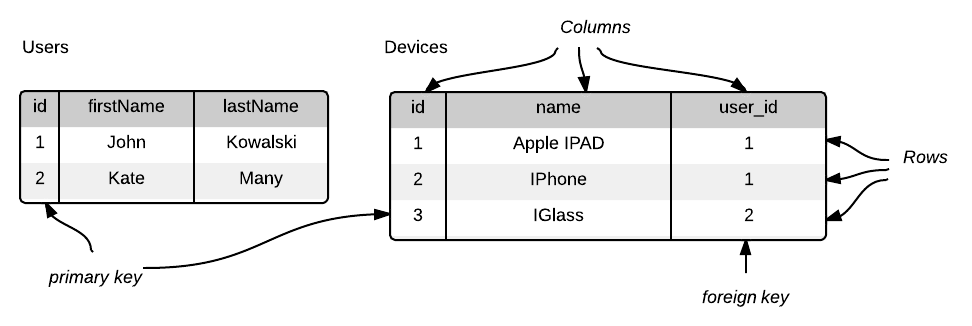
\includegraphics[width=0.7\paperwidth]{img/sql.png}
\end{center} 

}

\frame{\frametitle{No-relational database}  

\begin{itemize}
  \item information is represented as objects
  \item the objects are schema-less
  \item uses different models of store 
\end{itemize}  
 
\begin{center}
	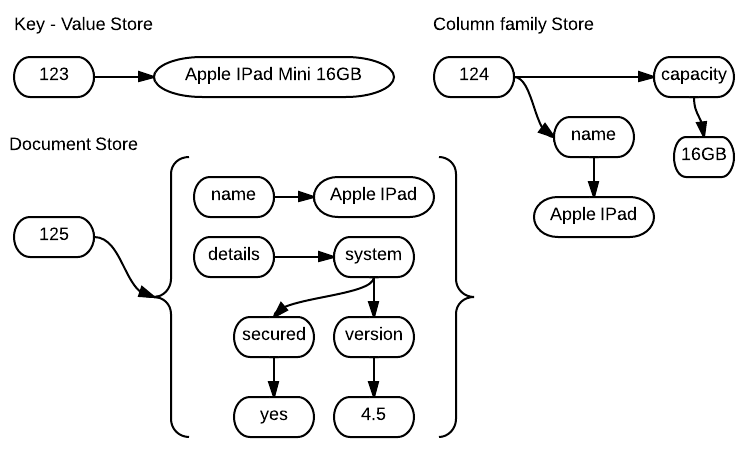
\includegraphics[width=0.6\paperwidth]{img/nosql.png}
\end{center}

}

\frame{\frametitle{No-relational database props}
	\begin{itemize}
	  \item Big data handling
	  \item Performance improvment 
	  \item Flexible data model
	  \item Scalability 
	\end{itemize} 
 
%A NoSQL database provides a mechanism for storage and retrieval of data that
%% use looser consistency models than traditional relational databases in order
% to achieve horizontal scaling and higher availability.

\vspace{1cm}

Examples:
\begin{itemize}
  \item Facebook - Casandra
  \item Google - Big Table
  \item Amazon - SimpleDB 
\end{itemize}

}

\section{Research questions and methods}  
\frame{\frametitle{Research questions and methods} 

Research questions
\begin{enumerate}
  \item What is the best architecture for large scale, high performance NoSQL databases?
  \item How to configure NoSQL databases to gain maximum efficiency?
  \item What are reading and writing response times for top used NoSQL databases?
  \item Which NoSQL database is the best for large scale, high performance database systems?
\end{enumerate}


Methods
\begin{itemize}
  \item Action Research - for finding out the best architecute of system and configuration of each database
  \item Experiment - for measuring reading/writing response times of each NoSQL databases on prepared architecture and configuration.
\end{itemize}

}

\section{Project plan}  
\frame{\frametitle{Project plan} 

\begin{enumerate}
  \item Choose the five most used NoSQL databases
	\begin{enumerate}
	  \item Find articles describing NoSQL databases
	  \item Choose five the most often used databases according to articles 
	\end{enumerate}
  \item Design an architecture of the system
	\begin{enumerate}
	  \item Find methods which are used for building large scale database systems
	  \item Find which methods ensure high performance
	  \item Use methods to design an architecture
	\end{enumerate}
  \item Find out the configuration for each database to be the most efficient on prepared architecture
    \begin{enumerate}
	  \item Find the optimization techniques for database dedicated systems
	  \item Find the database configuration to optimize operations on lots of data
	  \item For each database build system for designed architecture using prepared configuration
	\end{enumerate}
  \item Measure response times of each database
    \begin{enumerate}
      \item Prepare test suites
      \item Measure read and write time   
    \end{enumerate}  
\end{enumerate}

}

\section{Outcomes}
\frame{\frametitle{What is the best architecture for large scale, high performance NoSQL databases?}

\begin{itemize}
  \item many small servers instead of heavy ones
  \item two master to master servers for writing operations working in active/passive mode
  \item many server for reading operations working as slaves for masters
  \item load balancers int active/passive mode
  \item load balancers with healh check option
\end{itemize}

}

\frame{\frametitle{How to configure NoSQL databases to gain maximum efficiency?}

\begin{itemize}
  \item indexes on keys
  \item increased tcp socket limit to 64k
  \item 2GB memory per database server
  \item nodes connected using 1 Gigabit ethernet
  \item data should be stored on ssd drive
  \item usage of memory cache
\end{itemize}

}

\frame{\frametitle{Selected databses}
Top five databases extracted from literature:
	\begin{itemize}
	  \item MongoDB, CouchDB (Document store)
	  \item Voldemort, Redis (Key value store)
	  \item Cassandra (Column family store)
	\end{itemize}
}

\frame{\frametitle{Measure response times}

Measure assumptions:
\begin{itemize}
  \item database consists of 1 miltion different objects
  \item read / write action is counted as one operation
  \item we are interested in measuring how much read / write operation per
  second database can handle (database throughput)
  \item tests should be automatic
\end{itemize}
 
}

\frame{\frametitle{Which NoSQL database is the best for large scale, high
performance database systems?}

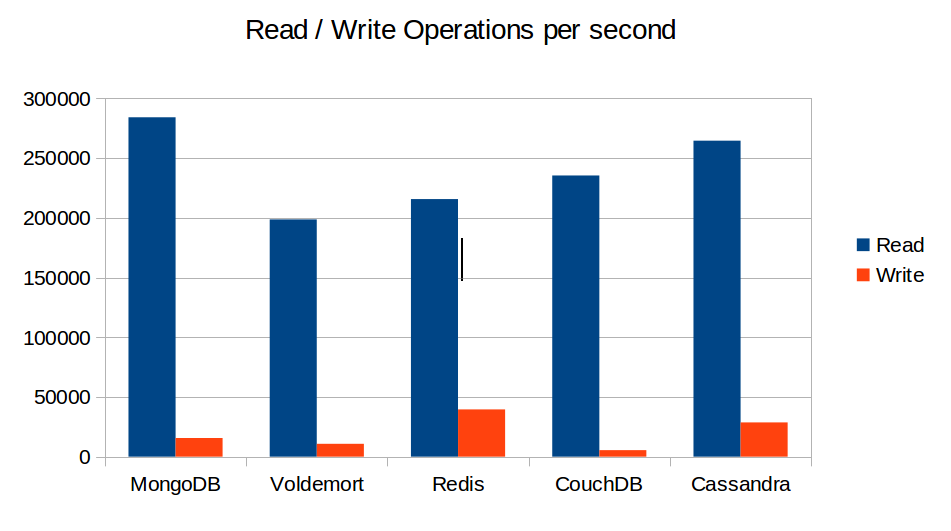
\includegraphics[width=0.9\paperwidth]{img/results.png} 

}

\section{Threats to validity}

\frame{\frametitle{Threats to validity}
\begin{itemize}
	\item choosed databases are the most used. There may exist better but not popular databases.
	\item to design architecture and prepare configuration we used documentation and articles. Results might be better if database experts would be involved
	\item machines used by us to perform load testing (bought in amazon cloud) might be distributed between many local networks. That would 
	cause decrease of performance and the results might be better in optimized environment
\end{itemize}

}

\section{References}
\frame{\frametitle{References}

\begin{thebibliography}{9}
\bibitem{asd}
Ludwik Kuzniarz
\emph{Lecture 5: Writing Project Proposal, Research Methodology course at WUT}. Blekinge Institute of Technology
 
\bibitem{qwe}  
Mateusz Bilski, Ireneusz Kawalec
\emph{Systematic Literature Review of Large Scale and High Performance NoSQL Databases in Web Applications}. Wroclaw University of Technology
  
  
\bibitem{zxc}  
\emph{List of NoSQL Databases. Access at 21.06.2013} \\
\url{http://nosql-database.org/}
\end{thebibliography}

}

\end{document}
